
\حصہ{تکونیاتی تفاعل}
اس حصہ میں ریڈیئن، تکونی تفاعل، دوریت اور بنیادی تکونی مماثل پر غور کیا جائے گا۔ 

\جزوحصہء{ریڈیئن}
چھوٹی جماعتوں میں زاویوں کو درجات کی صورت میں ناپا جاتا ہے۔ احصاء میں زاویہ کو ریڈیئن میں ناپا جاتا ہے جہاں \عددی{180^{\circ}} کو \عددی{\pi} ریڈیئن کہتے ہیں۔ریڈیئن کی استعمال سے حساب آسان ہو جاتا ہے۔

شکل \حوالہ{شکل_ابتدا_اکائی_دائرہ_ریڈیئن}-ا میں رداس \عددی{r} کا دائرہ دکھایا گیا ہے جس کے مرکز \عددی{C} سے دو شعاعیں نکل رہی ہیں جو مرکز پر وسطی زاویہ \عددی{\theta} بناتی ہیں۔یہ شعاعیں دائرے کو \عددی{A} اور \عددی{B} پر قطع کرتی ہیں۔قوس \عددی{AB} کی لمبائی \عددی{s} ہے۔اگر دائرے کا رداس \عددی{1} ہو تب ہم اس دائرے کو  \اصطلاح{اکائی دائرہ}\فرہنگ{اکائی!دائرہ}\حاشیہب{unit circle}\فرہنگ{unit!circle} کہتے ہیں۔اکائی دائرے پر اکائی لمبائی کا قوس جتنا زاویہ بناتی ہے اس کو ایک ریڈیئن زاویہ کہتے ہیں (یہی ایک ریڈیئن کی تعریف ہے)۔ شکل \حوالہ{شکل_ابتدا_اکائی_دائرہ_ریڈیئن}-ب میں ایک ریڈیئن کی اس تعریف کی وضاحت کی گئی ہے۔شکل \حوالہ{شکل_ابتدا_اکائی_دائرہ_ریڈیئن}-ج میں اکائی لمبائی کے دو قوس ساتھ ساتھ رکھے گئے ہیں جو ایک ایک ریڈیئن کا وسطی زاویہ بناتے ہیں۔یوں کل قوس کی لمبائی \عددی{2} ہے اور کل زاویہ \عددی{2} ریڈیئن ہے۔آپ دیکھ سکتے ہیں کہ اکائی دائرے پر وسطی زاویہ کی ریڈیئن میں ناپ قوس کی لمبائی کے برابر ہو گی۔شکل \حوالہ{شکل_ابتدا_اکائی_دائرہ_ریڈیئن}-د میں اس حقیقت کو دکھایا گیا ہے۔
\begin{figure}
\centering
\begin{subfigure}{0.25\textwidth}
\centering
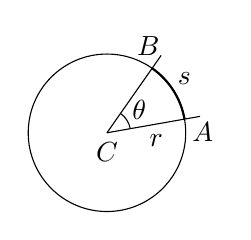
\begin{tikzpicture}
\draw(0,0) circle (1);
\draw(0,0)node[below]{$C$}--++(10:1.2)node[shift={(-80:0.2)}]{$A$}node[pos=0.5,shift={(-80:0.2)}]{$r$};
\draw(0,0)--++(55:1.2)node[shift={(145:0.2)}]{$B$};
\draw[thick] ([shift={(10:1)}]0,0) arc (10:55:1);
\draw[] ([shift={(10:0.3)}]0,0) arc (10:55:0.3);
\draw(0,0)++(35:0.5)node[]{$\theta$};
\draw(0,0)++(35:1.2)node[]{$s$};
\end{tikzpicture}
\caption{}
\end{subfigure}%
\begin{subfigure}{0.25\textwidth}
\centering
\begin{tikzpicture}
\draw(0,0) circle (1);
\draw(0,0)node[below]{$C$}--++(10:1.2)node[shift={(-80:0.2)}]{$A$}node[pos=0.5,shift={(-80:0.2)}]{$1$};
\draw(0,0)--++(55:1.2)node[shift={(145:0.2)}]{$B$};
\draw[thick] ([shift={(10:1)}]0,0) arc (10:55:1);
\draw[] ([shift={(10:0.3)}]0,0) arc (10:55:0.3);
\draw(0,0)++(35:0.5)node[]{$1$};
\draw(0,0)++(35:1.2)node[]{$1$};
\draw(-0.5,1)node[left]{\RL{اکائی دائرہ}};
\end{tikzpicture}
\caption{}
\end{subfigure}%
\begin{subfigure}{0.25\textwidth}
\centering
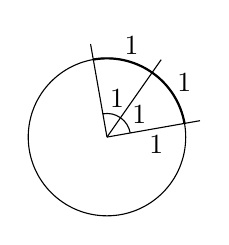
\begin{tikzpicture}
\draw(0,0) circle (1);
\draw(0,0)--++(10:1.2)node[pos=0.5,shift={(-80:0.2)}]{$1$};
\draw(0,0)--++(55:1.2);
\draw[thick] ([shift={(10:1)}]0,0) arc (10:55:1);
\draw[] ([shift={(10:0.3)}]0,0) arc (10:55:0.3);
\draw(0,0)++(35:0.5)node[]{$1$};
\draw(0,0)++(35:1.2)node[]{$1$};
\draw(0,0)--++(100:1.2);
\draw[thick] ([shift={(55:1)}]0,0) arc (55:100:1);
\draw[] ([shift={(55:0.3)}]0,0) arc (55:100:0.3);
\draw(0,0)++(75:0.5)node[]{$1$};
\draw(0,0)++(75:1.2)node[]{$1$};
\end{tikzpicture}
\caption{}
\end{subfigure}%
\begin{subfigure}{0.25\textwidth}
\centering
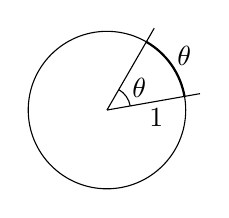
\begin{tikzpicture}
\draw(0,0) circle (1);
\draw(0,0)--++(10:1.2)node[pos=0.5,shift={(-80:0.2)}]{$1$};
\draw(0,0)--++(60:1.2);
\draw[thick] ([shift={(10:1)}]0,0) arc (10:60:1);
\draw[] ([shift={(10:0.3)}]0,0) arc (10:60:0.3);
\draw(0,0)++(35:0.5)node[]{$\theta$};
\draw(0,0)++(35:1.2)node[]{$\theta$};
\end{tikzpicture}
\caption{}
\end{subfigure}%
\caption{ریڈیئن کی تعریف}
\label{شکل_ابتدا_اکائی_دائرہ_ریڈیئن}
\end{figure}
%

زاویہ \عددی{ACB} کی ریڈیئن ناپ کی تعریف \ترچھا{اکائی دائرے} کی قوس \عددی{AB} کی لمبائی ہے۔چونکہ اکائی دائرے کا محیط \عددی{2\pi}  ہے اور ایک مکمل چکر \عددی{360^{\circ}} ہے لہٰذا درج ذیل تعلق لکھا جا سکتا ہے۔
\begin{align*}
\boxed{\pi\,\text{ریڈیئن}=180^{\circ}}
\end{align*}
%


\ابتدا{مثال}\شناخت{مثال_ابتدا_درجہ_ریڈیئن_الف}\موٹا{درجہ سے ریڈیئن میں زاویے کی تبدیلی}\\
\عددی{45^{\circ}} کو ریڈیئن میں لکھیں  اور \عددی{\tfrac{\pi}{6}} کو درجہ میں لکھیں۔\\
حل:\quad
شکل \حوالہ{شکل_مثال_ابتدا_درجہ_ریڈیئن_الف} دیکھیں۔
\begin{align*}
45\cdot\frac{\pi}{180}&=\frac{\pi}{4}\,\text{ریڈیئن}\\
\frac{\pi}{6}\cdot \frac{180}{\pi}&=30^{\circ}
\end{align*}
%
\begin{figure}
\centering
\begin{subfigure}{0.45\textwidth}
\centering
\begin{tikzpicture}[x={1.5cm},y={1.5cm},font=\small]
\draw(0,0)--++(1,0)--++(0,1)--(0,0);
\draw(0.5,0)node[below]{$1$} (1,0.5)node[right]{$1$};
\draw(45:1.4142/2)node[shift={(135:0.3cm)},]{$\sqrt{2}$};
\draw(0.35,0)node[above]{$45^{\circ}$};
\draw(1,1)++(-112.5:0.4)node[]{$45^{\circ}$};
\draw(1,0)node[shift={(-0.15,0.15)},]{$90^{\circ}$};
\begin{scope}[xshift=-2.5cm]
\draw(0,0)--++(1,0)--++(0,1)--(0,0);
\draw(0.5,0)node[below]{$1$} (1,0.5)node[right]{$1$};
\draw(45:1.4142/2)node[shift={(135:0.3cm)},]{$\sqrt{2}$};
\draw(22.5:0.4)node[]{$\tfrac{\pi}{4}$};
\draw(1,1)++(-112.5:0.4)node[]{$\tfrac{\pi}{4}$};
\draw(1,0)node[above left,]{$\tfrac{\pi}{2}$};
\end{scope}
\end{tikzpicture}
\end{subfigure}%
\begin{subfigure}{0.45\textwidth}
\centering
\begin{tikzpicture}[x={1.5cm},y={1.5cm},font=\small]
\draw(0,0)--++(1,0)--++(0,1.732)--(0,0);
\draw(0.5,0)node[below]{$1$} (1,0.866)node[right]{$\sqrt{3}$};
\draw(60:1)node[shift={(150:0.2cm)},]{$2$};
\draw(0.3,0)node[above,]{$60^{\circ}$};
\draw(1,1.732)++(-105:0.5)node[shift={(-0.05,-0.2)}]{$30^{\circ}$};
\draw(1,0)node[above left,]{$90^{\circ}$};
\begin{scope}[xshift=-2.5cm]
\draw(0,0)--++(1,0)--++(0,1.732)--(0,0);
\draw(0.5,0)node[below]{$1$} (1,0.866)node[right]{$\sqrt{3}$};
\draw(60:1)node[shift={(150:0.2cm)},]{$2$};
\draw(0.3,0)node[above,]{$\tfrac{\pi}{3}$};
\draw(1,1.732)++(-105:0.5)node[]{$\tfrac{\pi}{6}$};
\draw(1,0)node[above left,]{$\tfrac{\pi}{2}$};
\end{scope}
\end{tikzpicture}
\end{subfigure}
\caption{اشکال برائے مثال \حوالہ{مثال_ابتدا_درجہ_ریڈیئن_الف}}
\label{شکل_مثال_ابتدا_درجہ_ریڈیئن_الف}
\end{figure}
\انتہا{مثال}
%======================
\begin{mdframed}[frametitle={ریڈیئن اور درجہ}]
\begin{align*}
1^{\circ}&=\frac{\pi}{180}\approx 0.02 \,\text{ریڈیئن}\\
1\,\text{ریڈیئن}&=\frac{180}{\pi}\approx 57^{\circ}
\end{align*}
\end{mdframed}

دھیان رہے کہ زاویے کی پیمائش درجات میں ہونے کو \عددی{^{\circ}} کی علامت سے ظاہر کیا جاتا ہے جبکہ ریڈیئن کو بغیر علامت لکھا جاتا ہے۔یوں  \عددی{\theta=45^{\circ}}  سے مراد پینتالیس درجہ ہو گا جبکہ \عددی{\theta=3} سے مراد تین ریڈیئن ہو گا۔

\عددی{xy} مستوی میں شعاع کا راس مبدا پر اور شعاع کا ابتدائی مقام مثبت \عددی{x} محور پر ہونے کی صورت میں زاویہ کے مقام کو  \اصطلاح{معیاری مقام}\فرہنگ{معیاری!مقام}\حاشیہب{standard position}\فرہنگ{standard!position} کہتے ہیں۔مثبت \عددی{x} محور سے گھڑی کی  سوئی کے مخالف رخ زاویہ کی ناپ مثبت اور گھڑی کی سوئی کی رخ ناپ منفی تصور کی جاتی ہے (شکل \حوالہ{شکل_ابتدا_زاویہ_کی_ناپ})۔یوں مثبت \عددی{x} محور کا زاویہ \عددی{0} ریڈیئن اور منفی \عددی{x} محور کا زاویہ \عددی{\pi} ریڈیئن  ہو گا۔
\begin{figure}
\centering
\begin{tikzpicture}
\draw[-latex](-0.25,0)--(3,0)node[right]{$x$};
\draw[-latex](0,-0.2)--(0,2)node[above]{$y$};
\draw[-latex](0,0)--++(30:3);
\draw[-stealth]([shift={(0:0.8)}]0,0) arc (0:30:0.8);
\draw(20:0.8)node[right]{\RL{مثبت ناپ}}; 
\begin{scope}[xshift={-4cm},yshift={1cm}]
\draw[-latex](-2,0)--(1.5,0)node[right]{$x$};
\draw[-latex](0,-1.5)--(0,1)node[above]{$y$};
\draw[-latex](0,0)--++(-135:2);
\draw[-stealth]([shift={(0:0.8)}]0,0) arc (0:-135:0.8);
\draw(-60:0.8)node[right]{\RL{منفی ناپ}}; 
\end{scope}
\end{tikzpicture}
\caption{زاویے کی ناپ}
\label{شکل_ابتدا_زاویہ_کی_ناپ}
\end{figure}  

گھڑی مخالف چکر بیان کرتے ہوئے زاویے کی ناپ \عددی{2\pi} یعنی \عددی{360^{\circ}} سے زیادہ ہو سکتی ہے۔اسی طرح گھڑی کی رخ چکر بیان کرتے ہوئے زاویہ کی ناپ کچھ بھی ممکن ہے (شکل \حوالہ{شکل_ابتدا_زاویہ_ناپ})۔
\begin{figure}
\centering
\begin{subfigure}{0.25\textwidth}
\centering
\begin{tikzpicture}
\begin{axis}[small,clip=false,axis equal,width=4cm,axis lines=middle,xlabel={$x$},xlabel style={at={(current axis.right of origin)},anchor=west},ylabel style={at={(current axis.above origin)},anchor=south},ylabel={$y$},xtick={\empty},ytick={\empty},ymin=-0.75]
\addplot[mark=none,thick] plot coordinates {(0,0) ({2*cos(40)},{2*sin(40)})};
\addplot[-stealth,domain=0:400,samples=100]({(0.25+0.25/400*x)*cos(x)},{(0.25+0.25/400*x)*sin(x)})node[pos=0.8,below right]{$\tfrac{9\pi}{4}$};
\end{axis}
\end{tikzpicture}
\end{subfigure}%
\begin{subfigure}{0.25\textwidth}
\centering
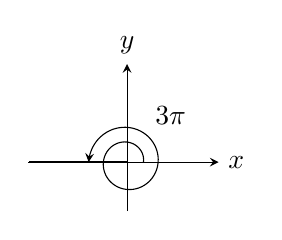
\begin{tikzpicture}
\begin{axis}[small,clip=false,axis equal,width=4cm,axis lines=middle,xlabel={$x$},xlabel style={at={(current axis.right of origin)},anchor=west},ylabel style={at={(current axis.above origin)},anchor=south},ylabel={$y$},xtick={\empty},ytick={\empty},ymin=-0.75,ymax=1.5]
\addplot[-stealth,domain=0:540,samples=100]({(0.25+0.25/400*x)*cos(x)},{(0.25+0.25/400*x)*sin(x)})node[pos=0.7,above right]{$3\pi$};
\draw[thick](axis cs:0,0)--(axis cs:-1.5,0);
\end{axis}
\end{tikzpicture}
\end{subfigure}%
\begin{subfigure}{0.25\textwidth}
\centering
\begin{tikzpicture}
\begin{axis}[small,clip=false,axis equal,width=4cm,axis lines=middle,xlabel={$x$},xlabel style={at={(current axis.right of origin)},anchor=west},ylabel style={at={(current axis.above origin)},anchor=south},ylabel={$y$},xtick={\empty},ytick={\empty},ymax=1]
\addplot[mark=none,thick] plot coordinates {(0,0) ({2*cos(-135)},{2*sin(-135)})};
\addplot[-stealth,domain=0:-135,samples=100]({(0.25-0.25/135*x)*cos(x)},{(0.25-0.25/135*x)*sin(x)})node[pos=0.7,below right]{$-\tfrac{3\pi}{4}$};
\end{axis}
\end{tikzpicture}
\end{subfigure}%
\begin{subfigure}{0.25\textwidth}
\centering
\begin{tikzpicture}
\begin{axis}[small,clip=false,axis equal,width=4cm,axis lines=middle,xlabel={$x$},xlabel style={at={(current axis.right of origin)},anchor=west},ylabel style={at={(current axis.above origin)},anchor=south},ylabel={$y$},xtick={\empty},ytick={\empty},ymax=1]
\addplot[-stealth,domain=0:-450,samples=100]({(0.25-0.25/450*x)*cos(x)},{(0.25-0.25/450*x)*sin(x)})node[pos=0.6,above right]{$-\tfrac{5\pi}{2}$};
\draw[thick](axis cs:0,0)--(axis cs:0,-1);
\end{axis}
\end{tikzpicture}
\end{subfigure}%
\caption{مثبت اور منفی ریڈیئن}
\label{شکل_ابتدا_زاویہ_ناپ}
\end{figure}

شکل \حوالہ{شکل_ابتدا_جسامت_اور_زاویہ}-ا میں چند اشکال  کو لچکدار \عددی{xy} مستوی پر دکھایا گیا ہے۔اس \عددی{xy} مستوی کو کھینچ کر \عددی{x} رخ اور \عددی{y} رخ کی لمبائیاں \عددی{k} گنا کرنے سے  شکل \حوالہ{شکل_ابتدا_جسامت_اور_زاویہ}-ب حاصل ہوتا ہے۔ہم کہتے ہیں کہ  جسامت \عددی{k} گنا کر دی گئی ہے۔یوں اگر بائیں شکل کے تکون کی افقی اور انتصابی اطراف کی لمبائیاں بالترتیب \عددی{a} اور \عددی{b} ہوں تب اس کی وتر کی لمبائی \عددی{\sqrt{a^2+b^2}} ہو گی۔دائیں شکل میں تکون کی افقی اور انتصابی اطراف کی لمبائیاں بالترتیب \عددی{ka} اور \عددی{kb} ہوں گی لہٰذا اس کا وتر \عددی{\sqrt{(ka)^2+(kb)^2}=k\sqrt{a^2+b^2}} ہو گا۔آپ نے دیکھا کہ دائیں مستوی پر نا صرف افقی اور انتصابی خط بلکہ ترچھے خط کی لمبائی بھی \عددی{k} گنا ہو گئی ہے۔چونکہ ہر ترچھے خط کو کسی تکون کا وتر تصور کیا جا سکتا ہے لہٰذا دائیں مستوی پر (ہر افقی اور ہر انتصابی خط کے ساتھ ساتھ) ہر ترچھے خط کی لمبائی \عددی{k} گنا ہو گی۔کیا جسامت \عددی{k} گنا  کرنے سے لمبائی قوس بھی \عددی{k} گنا ہو گی؟ اس کا جواب ہے "جی ہاں" جس کا ثبوت اب پیش کرتے ہیں۔
\begin{figure}
\centering
\begin{tikzpicture}[x=0.75cm,y=0.75cm]
\draw[-latex](-1.25,0)--(2.5,0)node[right]{$x$};
\draw[-latex](0,-0.2)--(0,1.25)node[above]{$y$};
\draw(1,0) circle (0.75);
\draw(2,0)--(2,1)--(0,0);
\draw(0,0)--(-0.75,1);
\draw(-0.2,0.6)node[]{$\alpha$};
\draw(-0.6,0.3)node[]{$\beta$};
\RightAngle{(2,1)}{(2,0)}{(2.5,0)};
\draw(-0.5,-0.5)node[]{(ا)};
\begin{scope}[x={1.5cm},y={1.5cm},xshift={-6cm}]
\draw[-latex](-1.25,0)--(2.5,0)node[right]{$x$};
\draw[-latex](0,-0.2)--(0,1.25)node[above]{$y$};
\draw(1,0) circle (0.75);
\draw(2,0)--(2,1)--(0,0);
\draw(0,0)--(-0.75,1);
\draw(-0.1,0.3)node[]{$\alpha$};
\draw(-0.3,0.15)node[]{$\beta$};
\RightAngle{(2,1)}{(2,0)}{(0,0)};
\draw(-0.5,-0.5)node[]{(ب)};
\end{scope}
\end{tikzpicture}
\caption{شکل بڑھانے یا گھٹانے کا زاویہ پر اثر نہیں پایا جاتا ہے۔}
\label{شکل_ابتدا_جسامت_اور_زاویہ}
\end{figure}

\begin{figure}
\centering
\begin{minipage}{0.45\textwidth}
\centering
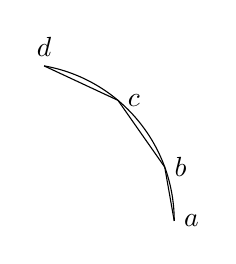
\begin{tikzpicture}
\draw([shift={(0:2)}]0,0) arc (0:80:2);
\coordinate (kA) at (0:2);
\coordinate (kB) at (20:2);
\coordinate (kC) at (50:2);
\coordinate (kD) at (80:2);
\draw(kA)node[right]{$a$}--(kB)node[right]{$b$}--(kC)node[right]{$c$}--(kD)node[above]{$d$};
\end{tikzpicture}
\caption{قوس کی لمبائی}
\label{شکل_ابتدا_قوس_لمبائی}
\end{minipage}\hfill
\begin{minipage}{0.45\textwidth}
\centering
\centering
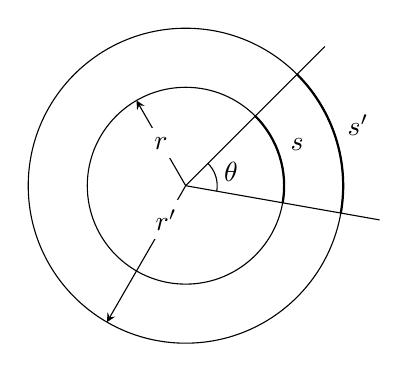
\begin{tikzpicture}
\draw(0,0) circle (1.25);
\draw(0,0) circle (2);
\draw(0,0)--++(-10:2.5);
\draw(0,0)--++(45:2.5);
\draw[thick]([shift={(-10:1.25)}]0,0) arc (-10:45:1.25);
\draw[thick]([shift={(-10:2)}]0,0) arc (-10:45:2);
\draw([shift={(-10:0.4)}]0,0) arc (-10:45:0.4);
\draw(17:0.6)node[]{$\theta$};
\draw(15:2)node[above right]{$s'$};
\draw(15:1.25)node[above right]{$s$};
\draw[-stealth](0,0)--++(120:1.25)node[pos=0.5,fill=white]{$r$};
\draw[-stealth](0,0)--++(-120:2)node[pos=0.25,fill=white]{$r'$};
\end{tikzpicture}
\caption{محیط دائرہ}
\label{شکل_ابتدا_دائرہ_اور_ریڈیئن}
\end{minipage}%
\end{figure}

شکل \حوالہ{شکل_ابتدا_قوس_لمبائی} میں قوس کی لمبائی جاننے کی خطر قوس پر مختلف نقطے منتخب کرتے ہوئے ان کے بیچ سیدھے خط کھینچے گئے ہیں۔ان سیدھے خطوط کی مجموعی لمبائی کو قوس کی تخمینی لمبائی لی جا سکتی ہے۔آپ دیکھ سکتے ہیں کہ قوس پر نقطوں کی تعداد بڑھا کر اس کو زیادہ ٹکڑوں میں تقسیم کرتے ہوئے قوس کی لمبائی اور سیدھے خطوط کی مجموعی لمبائی میں فرق کو ہم جتنا چاہیں کم کر سکتے ہیں۔اب اگر اس قوس کی جسامت کو \عددی{k} گنا کیا جائے تب ہر سیدھے خط کی لمبائی \عددی{k} گنا ہو گی لہٰذا ان کی مجموعی لمبائی (جو قوس کی لمبائی ہے) بھی \عددی{k} گنا ہو گی۔(ثبوت مکمل ہوا۔)


شکل \حوالہ{شکل_ابتدا_قوس_زاویہ_رداس}-ا میں رداس \عددی{r} کے دائرے پر قوس \عددی{s} اور وسطی زاویہ \عددی{\theta} دکھائے گئے ہیں۔اس دائرے کے مرکز پر ہم \عددی{1} رداس کا دائرہ بناتے ہیں (شکل \حوالہ{شکل_ابتدا_قوس_زاویہ_رداس}-ب؛ اگر دیے گئے دائرے کا رداس اکائی سے کم ہو تب یہ دائرہ اکائی دائرے کے اندر نظر آئے گا)۔ (جیسا شکل \حوالہ{شکل_ابتدا_قوس_زاویہ_رداس}-ب میں دکھایا گیا ہے) ریڈیئن کی تعریف کی رو سے اکائی دائرے پر قوس اور زاویہ آپس میں برابر ہوں گے۔شکل \حوالہ{شکل_ابتدا_قوس_زاویہ_رداس}-ب میں دونوں دائروں پر  قوس کی لمبائیوں کا تناسب \عددی{\tfrac{s}{\theta}} اور دائروں کے رداس کی لمبائیوں کا تناسب \عددی{\tfrac{r}{1}} ایک جیسا ہوں گے، یعنی \عددی{\tfrac{s}{\theta}=\tfrac{r}{1}} جس سے درج ذیل اہم ترین کلیہ ملتا ہے۔
\begin{mdframed}[frametitle={قوس، رداس اور زاویے کا تعلق}]
\begin{align*}
s=r\theta
\end{align*}
\end{mdframed}
%
\begin{figure}
\centering
\begin{subfigure}{0.45\textwidth}
\centering
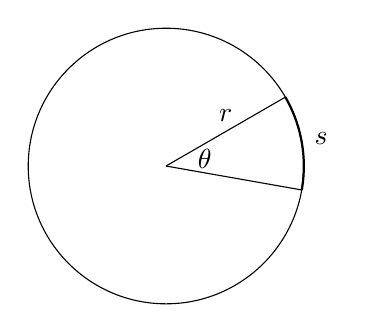
\begin{tikzpicture}
\draw (0,0) circle (1.75);
\draw(0,0)--++(-10:1.75);
\draw(0,0)--++(30:1.75)node[pos=0.5,above]{$r$};
\draw[thick]([shift={(-10:1.75)}]0,0) arc (-10:30:1.75);
\draw(10:0.5)node[]{$\theta$};
\draw(10:2)node[]{$s$};
\end{tikzpicture}
\end{subfigure}%
\begin{subfigure}{0.45\textwidth}
\centering
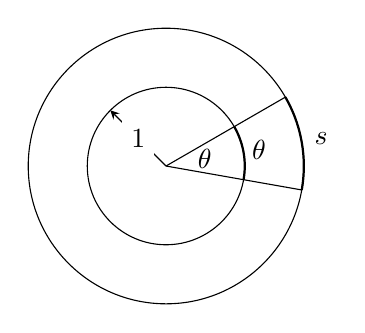
\begin{tikzpicture}
\draw (0,0) circle (1) circle (1.75);
\draw(0,0)--++(-10:1.75);
\draw(0,0)--++(30:1.75);
\draw[-stealth](0,0)--++(135:1)node[pos=0.5,fill=white]{$1$};
\draw[thick]([shift={(-10:1)}]0,0) arc (-10:30:1);
\draw[thick]([shift={(-10:1.75)}]0,0) arc (-10:30:1.75);
\draw(10:0.5)node[]{$\theta$};
\draw(10:1.2)node[]{$\theta$};
\draw(10:2)node[]{$s$};
\end{tikzpicture}
\end{subfigure}%
\caption{قوس، رداس اور زاویے کا تعلق۔}
\label{شکل_ابتدا_قوس_زاویہ_رداس}
\end{figure}
% 
\begin{mdframed}[frametitle={زاویہ ناپنے کی روایت: ریڈیئن استعمال کریں}]
یہاں کے بعد اس کتاب میں زاویے کو ریڈیئن میں ناپا جائے گا۔جہاں زاویے کو ریڈیئن میں نہیں ناپا گیا ہو وہاں صریحاً بتلایا جائے گا۔یوں اگر ہم زاویہ \عددی{\tfrac{\pi}{6}} کی بات کریں تب اس سے مراد \عددی{\tfrac{\pi}{6}} ریڈیئن کا زاویہ ہو گا نا کہ \عددی{\tfrac{\pi}{6}} درجے کا زاویہ۔
\end{mdframed}

\ابتدا{مثال}
رداس \عددی{8} کے دائرے پر غور کریں۔ (الف) دائرے پر \عددی{2\pi} لمبائی کا قوس، دائرے کے مرکز پر کیا وسطی زاویہ بناتا ہے۔ (ب) اس قوس کی لمبائی تلاش کریں جو 
\عددی{\tfrac{3\pi}{4}} وسطی زاویہ بناتا ہو۔\\
حل:\quad
\begin{gather*}
\begin{aligned}
 s=r\theta=8(\tfrac{3\pi}{4})=6\pi \quad \text{(ب)}
\end{aligned}\quad\quad
\begin{aligned}
\theta=\frac{s}{r}=\frac{2\pi}{8}=\frac{\pi}{4} \quad \text{(الف)}
\end{aligned}
\end{gather*} 
\انتہا{مثال}
%================================

\جزوحصہء{چہ بنیادی تکونیاتی تفاعل}
آپ  زاویہ حادہ کے تکونیاتی تفاعل سے بخوبی واقف ہوں گے جو قائمہ مثلث کے اطراف کی لمبائیوں کی تناسب سے حاصل ہوتے ہیں (شکل \حوالہ{شکل_ابتدا_قائمہ_مثلث})۔ ہم انہیں تعریف کو وسعت دیتے ہوئے  زاویہ منفرجہ اور منفی زاویوں پر بھی لاگو کرتے ہیں جہاں معیاری مقام پر رداس \عددی{r} کے دائرے میں زاویہ پایا جاتا ہے۔ہم اب ان تکونیاتی تفاعل کو نقطہ \عددی{N(x,y)} کے محدد کی صورت میں بیان کرتے ہیں جہاں مبدا سے خارج ہوتا ہوا شعاع دائرے کو \عددی{N(x,y)} پر قطع کرتا ہے۔
\begin{figure}
\centering
\begin{minipage}[b][][b]{0.3\textwidth}
\centering
\begin{tikzpicture}
\path[name path=kX](0,0)--(3,0);
\draw(0,0)--++(30:2)coordinate(kA);
\draw(kA)--($(0,0)!(kA)!(3,0)$)coordinate(kB)--(0,0);
\RightAngle{(0,0)}{(kB)}{(kA)};
\draw[-stealth]([shift={(0:0.6)}]0,0) arc (0:30:0.6);
\draw(14:0.8)node[]{$\theta$};
\draw($(0,0)!0.5!(kB)$)node[below]{قاعدہ};
\draw($(kA)!0.5!(kB)$)node[right]{عمود};
\draw($(0,0)!0.5!(kA)$)node[above]{وتر};
\end{tikzpicture}
\end{minipage}\hfill
\begin{minipage}[b][][b]{0.66\textwidth}
\begin{gather*}
\begin{aligned}
\sin \theta&=\tfrac{\text{عمود}}{\text{وتر}},\\
\cos \theta&=\tfrac{\text{قاعدہ}}{\text{وتر}},\\
\tan \theta&=\tfrac{\text{عمود}}{\text{قاعدہ}},
\end{aligned}\quad
\begin{aligned}
\csc&=\tfrac{\text{وتر}}{\text{عمود}}\\
\sec&=\tfrac{\text{وتر}}{\text{قاعدہ}}\\
\cot&=\tfrac{\text{قاعدہ}}{\text{عمود}}
\end{aligned}
\end{gather*}
\end{minipage}%
\caption{قائمہ مثلث اور تکونیاتی تفاعل}
\label{شکل_ابتدا_قائمہ_مثلث}
\end{figure}

شکل \حوالہ{شکل_ابتدا_تفاعل_تکونیاتی}-ا کو دیکھتے ہوئے ان تفاعل کو یہاں پیش کرتے ہیں۔
\begin{figure}
\centering
\begin{subfigure}{0.45\textwidth}
\centering
\begin{tikzpicture}
\draw[-latex](-1.5,0)--(2,0)node[right]{$x$};
\draw[-latex](0,-1.25)--(0,1.5)node[above]{$y$};
\draw(0,0)node[below left]{$M$} circle (1);
\draw[-latex](0,0)--++(135:1.7);
\draw[-stealth]([shift={(0:0.3)}]0,0) arc (0:135:0.3);
\draw(45:0.5)node[]{$\theta$};
\draw(135:1)node[circ]{}node[left]{$N(x,y)$};
\draw(135:0.6)node[shift={(45:0.2)}]{$r$};
\draw(1,0)node[below right]{$r$};
\end{tikzpicture}
\caption{}
\end{subfigure}%
\begin{subfigure}{0.45\textwidth}
\centering
\begin{tikzpicture}
\draw[-latex](-1.5,0)--(2,0);
\draw[-latex](0,-1.25)--(0,1.5);
\draw(0,0)node[below left]{$M$} circle (1);
\draw[-latex](0,0)--++(55:1.7);
\draw[-stealth]([shift={(0:0.3)}]0,0) arc (0:55:0.3);
\draw(24:0.45)node[font=\small]{$\theta$};
\draw(55:1)node[circ]{}node[right,xshift={1mm}]{$N(x,y)$}coordinate(kA);
\draw[thick](0,0)--++(55:1);
\draw(55:0.6)node[shift={(145:0.15)}]{$r$};
\draw(1,0)node[below right]{$r$};
\draw[dashed,thick](kA)--($(0,0)!(kA)!(1.5,0)$)node[pos=0.6,right,font=\small]{$y$}coordinate(kB);
\draw[thick](0,0)--(kB)node[pos=0.5,below]{$x$};
\end{tikzpicture}
\caption{}
\end{subfigure}%
\caption{تکونیاتی تفاعل}
\label{شکل_ابتدا_تفاعل_تکونیاتی}
\end{figure}

\begin{mdframed}[frametitle={چہ تکونیاتی تفاعل}]
\begin{gather*}
\begin{aligned}
\text{سائن}\quad \sin \theta&=\frac{y}{r}\\
\text{کوسائن}\quad \cos \theta&=\frac{x}{r}\\
\text{ٹینجنٹ}\quad \tan \theta&=\frac{y}{x}
\end{aligned}\quad\quad
\begin{aligned}
\text{کوسیکنٹ}\quad \csc \theta&=\frac{r}{y}\\
\text{سیکنٹ}\quad \sec \theta&=\frac{r}{x}\\
\text{کوٹینجنٹ}\quad \cot \theta&=\frac{x}{y}
\end{aligned}
\end{gather*}
\end{mdframed}

آپ شکل \حوالہ{شکل_ابتدا_تفاعل_تکونیاتی}-ب سے دیکھ سکتے ہیں کہ زاویہ حادہ کی صورت میں تکونیاتی تفاعل کی توسیعی تعریف اور قائمہ زاویہ تکونی تعریف ایک جیسے ہیں۔ 

جیسا آپ دیکھ سکتے ہیں \عددی{x=0} کی صورت میں \عددی{\tan \theta} اور \عددی{\sec \theta} غیر معین ہیں (چونکہ کسی بھی عدد کو صفر سے تقسیم نہیں کیا جا سکتا ہے)۔یوں یہ \عددی{\theta=\mp\tfrac{\pi}{2},\mp\tfrac{3\pi}{2},\cdots} کے لئے غیر معین ہیں۔اسی طرح \عددی{y=0} یعنی \عددی{\theta=0,\mp \pi, \mp 2\pi,\cdots} کے لئے \عددی{\cot \theta} اور \عددی{\csc \theta} غیر معین ہیں۔

اسی طرح درج ذیل تعریف بھی لکھے جا سکتے ہیں۔
\begin{mdframed}[frametitle={تکونیاتی تفاعل کے باہمی تعلقات}]
\begin{align*}
\tan\theta&=\frac{\sin\theta}{\cos\theta}&\cot\theta&=\frac{1}{\tan\theta}\\
\sec\theta&=\frac{1}{\cos\theta}& \csc\theta&=\frac{1}{\sin\theta}
\end{align*}
\end{mdframed}

مستوی میں نقطہ \عددی{N(x,y)} کو مبدا سے فاصلہ \عددی{r} اور زاویہ \عددی{\theta} کی صورت میں لکھا جا سکتا ہے (شکل \حوالہ{شکل_ابتدا_کارتیسی_رداس_زاویہ})۔چونکہ \عددی{\cos\theta=\tfrac{x}{r}} اور \عددی{\sin\theta=\tfrac{y}{r}} ہیں لہٰذا درج ذیل ہو گا۔
\begin{align*}
x=r\cos\theta,\quad y=r\sin\theta
\end{align*}
%
\begin{figure}
\centering
\begin{minipage}{0.45\textwidth}
\centering
\begin{tikzpicture}
\draw[-latex](-1.25,0)--(1.5,0)node[right]{$x$};
\draw[-latex](0,-1.2)--(0,1.5)node[above]{$y$};
\draw(0,0)node[below left]{$M$} circle (1);
\draw[-latex,thick](0,0)--(160:1.5)node[pos=0.33,shift={(70:0.2)}]{$r$};
\draw(160:1)node[circ]{} ++(0,0.1)--++(-0.5,0.5)node[above,xshift={-0.5cm},font=\footnotesize]{$N(x,y)=(r\cos\theta,r\sin\theta)$};
\draw[-stealth]([shift={(0:0.3)}]0,0) arc (0:160:0.3);
\draw(45:0.5)node[]{$\theta$};
\end{tikzpicture}
\caption{مستوی میں کارتیسی محدد کا $r$ اور $\theta$ میں اظہار۔}
\label{شکل_ابتدا_کارتیسی_رداس_زاویہ}
\end{minipage}\hfill
\begin{minipage}{0.45\textwidth}
\begin{tikzpicture}
\draw[-latex](-1.25,0)--(1.5,0)node[right]{$x$};
\draw[-latex](0,-1.2)--(0,1.5)node[above]{$y$};
\draw(0,0) circle (1);
\draw[thick](0,0)--(120:1)node[pos=0.6,shift={(30:0.2)}]{$1$}coordinate(kA);
\draw(kA)++(-0.05,0.05)--++(-0.5,0.25)node[above,xshift={-0.5cm},font=\footnotesize]{$N(x,y)=(\cos\theta,\sin\theta)$};
\draw[-stealth]([shift={(0:0.3)}]0,0) arc (0:120:0.3);
\draw(45:0.5)node[]{$\theta$};
\draw(kA)--($(0,0)!(kA)!(1,0)$)coordinate(kB)node[pos=0.6,left,xshift={1mm},font=\footnotesize]{$\abs{y}$};
\draw($(kB)!0.5!(0,0)$)node[below,font=\footnotesize]{$\abs{x}$};
\shade[lgray] (0,0)--(kA)--(kB)--(0,0);
\end{tikzpicture}
\caption{زاویہ $\theta$ کے لئے زاویہ حادہ تکون}
\label{شکل_ابتدا_تکون_زاویہ_حادہ}
\end{minipage}\hfill
\end{figure}

\جزوحصہء{تکونیاتی تفاعل کی قیمتیں}
شکل \حوالہ{شکل_ابتدا_تفاعل_تکونیاتی} کے دائرے میں \عددی{r=1} ہونے کی صورت میں \عددی{\sin\theta} اور \عددی{\cos\theta} کی تعارفی مساوات درج ذیل صورت اختیار کرتی ہیں۔
\begin{align*}
\cos\theta=x,\quad \sin\theta=y
\end{align*}
یوں ہم سائن اور کوسائن کی قیمتوں کو بالترتیب نقطہ \عددی{N(x,y)} کی \عددی{x} اور \عددی{y} محدد سے پڑھ سکتے ہیں۔نقطہ \عددی{N} سے \عددی{x} محور پر قائمہ گراتے ہوئے حاصل حوالہ تکون سے بھی انہیں حاصل کیا جا سکتا ہے (شکل \حوالہ{شکل_ابتدا_تکون_زاویہ_حادہ})۔ہم \عددی{x} اور \عددی{y} کی قیمتیں تکون کی اطراف سے ناپتے ہیں۔\عددی{x} اور \عددی{y} کی علامتیں اس ربع سے تعین کی جاتی ہیں جس میں تکون پایا جاتا ہو۔

\ابتدا{مثال}\شناخت{مثال_ابتدا_تکونیاتی_قیمتیں_الف}
\عددی{\tfrac{2\pi}{3}} ریڈیئن کا سائن اور کوسائن تلاش کریں۔\\
حل:\quad
\موٹا{پہلا قدم}\quad
زاویے کو معیاری مقام پر اکائی دائرے میں بنائیں۔حوالہ  تکون کے اطراف کی لمبائیاں لکھیں (شکل \حوالہ{شکل_مثال_ابتدا_تکونیاتی_قیمتیں_الف})۔\\
\موٹا{دوسرا قدم}\quad
جہاں اکائی دائرے کو شعاع قطع کرتی ہے اس نقطے کے محدد دریافت کریں:
\begin{align*}
\cos\frac{2\pi}{3}&=x\,\text{\RL{کا محدد}} \,N=-\frac{1}{2}\\
\sin\frac{2\pi}{3}&=y\,\text{\RL{کا محدد}} \,N=\frac{\sqrt{3}}{2}\\
\end{align*}
%
\begin{figure}
\centering
\begin{minipage}{0.45\textwidth}
\centering
\begin{tikzpicture}[x={1.2cm},y={1.2cm}]
\draw[-latex](-1.25,0)--(1.25,0)node[right]{$x$};
\draw[-latex](0,-1.1)--(0,1.2)node[right]{$y$};
\draw(0,0) circle (1);
\draw(0,0)--++(120:1)coordinate(kA);
\draw[-stealth]([shift={(0:0.3)}]0,0) arc (0:120:0.3);
\draw(45:0.5)node[]{$\tfrac{2\pi}{3}$};
\draw(kA)--($(0,0)!(kA)!(-1,0)$)coordinate(kB)node[pos=0.6,left,xshift={0.5mm}]{$\tfrac{\sqrt{3}}{2}$};
\draw($(kB)!0.5!(0,0)$)node[below]{$\tfrac{1}{2}$};
\draw(kA)++(100:0.1)--++(100:0.5)node[above]{$(\cos\tfrac{2\pi}{3},\sin\tfrac{2\pi}{3})=(-\tfrac{1}{2},\tfrac{\sqrt{3}}{2})$};
\end{tikzpicture}
\caption{تکونیاتی تفاعل کی قیمتیں (مثال \حوالہ{مثال_ابتدا_تکونیاتی_قیمتیں_الف})}
\label{شکل_مثال_ابتدا_تکونیاتی_قیمتیں_الف}
\end{minipage}\hfill
\begin{minipage}{0.45\textwidth}
\centering
\begin{tikzpicture}[x={1.2cm},y={1.2cm}]
\draw[-latex](-1.25,0)--(1.25,0)node[right]{$x$};
\draw[-latex](0,-1.12)--(0,1.2)node[above]{$y$};
\draw(0.6,0.5)node[above]{$A$}node[below]{\RL{تمام مثبت}};
\draw(-0.6,0.5)node[above]{$S$}node[below]{\RL{سائن مثبت}};
\draw(-0.6,-0.5)node[above]{$T$}node[below]{\RL{ٹینجنٹ مثبت}};
\draw(0.6,-0.5)node[above]{$C$}node[below]{\RL{کوسائن مثبت}};
\end{tikzpicture}
\caption{قاعدہ $CAST$}
\label{شکل_ابتدا_تکونیاتی_علامت}
\end{minipage}\hfill
\end{figure}

تکونیاتی تفاعل کی قیمتوں کی علامت جاننے کے لئے  شکل \حوالہ{شکل_ابتدا_تکونیاتی_علامت} میں دکھایا گیا \عددی{CAST} کا قاعدہ یاد رکھیں۔
\انتہا{مثال}
%========================
\ابتدا{مثال}\شناخت{مثال_ابتدا_منفی_زاویہ_تکونی}
\عددی{-\tfrac{\pi}{4}} ریڈیئن کا سائن اور کوسائن تلاش کریں۔\\
حل:\quad
\موٹا{پہلا قدم:}\quad
معیاری مقام پر اکائی دائرے میں زاویہ کھینچ کر حوالہ تکون کے اطراف کی لمبائیاں لکھیں (شکل \حوالہ{شکل_مثال_ابتدا_منفی_زاویہ_تکونی})۔\\
\موٹا{دوسرا قدم:}\quad
نقطہ \عددی{N} کے محدد تلاش کریں۔
\begin{align*}
\cos(-\tfrac{\pi}{4})&=x\,\text{\RL{کا محدد}}\,N=\frac{\sqrt{2}}{2}\\
\sin(-\tfrac{\pi}{4})&=y\,\text{\RL{کا محدد}}\,N=-\frac{\sqrt{2}}{2}
\end{align*}
%
\begin{figure}
\centering
\begin{tikzpicture}
\draw[-latex](-1.25,0)--(1.25,0)node[right]{$x$};
\draw[-latex](0,-1.2)--(0,1.2)node[above]{$y$};
\draw(0,0) circle (1)node[pos=0.4,below left]{$1$};
\draw(0,0)--++(-45:1)coordinate(kA)node[below right]{$N:[\cos (-\tfrac{\pi}{4}),\sin(-\tfrac{\pi}{4})]=(\tfrac{\sqrt{2}}{2},-\tfrac{\sqrt{2}}{2})$};
\draw[-stealth]([shift={(0:0.3)}]0,0) arc (0:-45:0.3);
\draw(-22:0.55)node[font=\footnotesize]{$-\tfrac{\pi}{4}$};
\draw(kA)--($(0,0)!(kA)!(1,0)$)coordinate(kB)node[pos=0.5,right,fill=white,font=\footnotesize]{$\tfrac{\sqrt{2}}{2}$};
\draw($(kB)!0.5!(0,0)$)node[above,font=\footnotesize]{$\tfrac{\sqrt{2}}{2}$};
\end{tikzpicture}
\caption{شکل برائے مثال \حوالہ{مثال_ابتدا_منفی_زاویہ_تکونی}}
\label{شکل_مثال_ابتدا_منفی_زاویہ_تکونی}
\end{figure}
\انتہا{مثال}
%========================

درج بالا دو مثالوں کی طرح حل کرتے ہوئے جدول میں دیے قیمتیں حاصل کی جا سکتی ہیں۔
\begin{table}
\centering
\begin{otherlanguage}{english}
\begin{tabular}{CCCCCC}
\text{\urdufont{درجہ}} & 0^{\circ} &30^{\circ}&45^{\circ}&60^{\circ}&90^{\circ}\\
\text{\urdufont{ریڈیئن}}&0&\frac{\pi}{6}&\frac{\pi}{4}&\frac{\pi}{3}&\frac{\pi}{2}\\
\hline
\sin \theta&0&\tfrac{1}{2}&\frac{\sqrt{2}}{2}&\frac{\sqrt{3}}{2}&1\\
\cos\theta&1&\frac{\sqrt{3}}{2}&\frac{\sqrt{2}}{2}&\tfrac{1}{2}&0\\
\tan\theta&0&\frac{1}{\sqrt{3}}&1&\sqrt{3}&
\end{tabular}
\end{otherlanguage}
\end{table}
